% Brief overview of the observables that are measured
The observables we measured in the $1 + 1$D CDT model are the \emph{standard deviation} of the length profile $\sigma_\ell$ and the \emph{length correlation} $\rho_\ell(t)$ as introduced in section \ref{sec:observables}.
In this section we will present and discuss the results found for these observables.

\subsection{Pre-analysis}
% Determination of the equilibration time and correlation time
Before the actual measurements can be performed some data analysis need to be done beforehand.

\paragraph{Equilibration}
To be able to take measurements of the wanted observables in the Markov-chain Monte Carlo simulation the system needs to be thermalised. Which is to say that the system should be in a `typical' state, such that the expectation value of an observable at any timestep in the simulation is the same as any other.
We start the system in a non-typical, flat spacetime, so it takes some Markov-chain steps before the system is in equilibrium.
We want to only start measurements after this \emph{equilibration time}, so we need to estimate it to know when to start measuring.

Preferably one used the observable of interest to determine the equilibration time, however it is very difficult to quantify when a function like $\rho_\ell(t)$ has thermalised. So we determine the equilibration time using $\sigma_\ell$.
To determine when the system has equilibrated in terms of $\sigma_\ell$ we fit a function which converges exponentially towards the average value:
$\sigma(t) = \hat\sigma \qty(1 - e^{t/t_\text{eq}})$, where $t$ here is the Monte Carlo simulation time.
This works well because the initial state is flat thus having $\sigma_\ell = 0$, which over time goes towards some mean value and fluctuates around it.
This fitting procedure is visualised in Fig. \ref{fig:thermalisation}.
\begin{figure}[h]
    \centering
    \begin{minipage}[t]{0.47\linewidth}
        \centering
        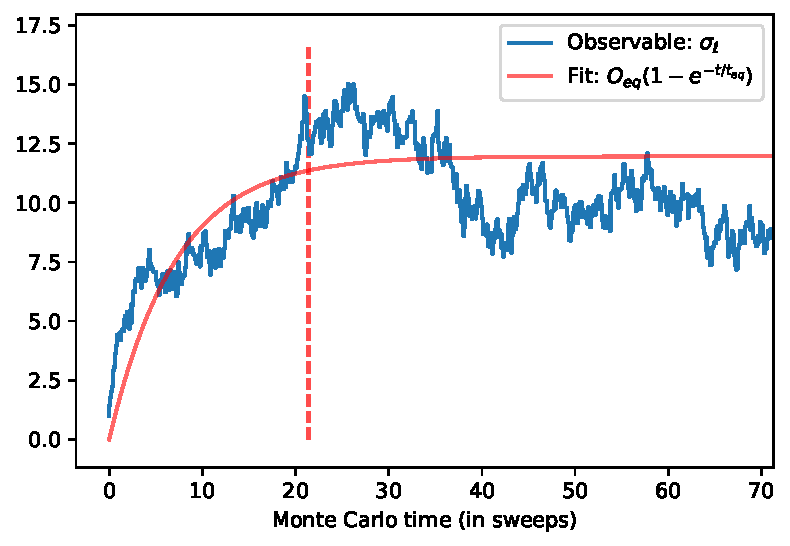
\includegraphics[width=0.95\linewidth]{img/teq_thermalisation.pdf}
        \caption{Visualisation of determination of thermalisation by fitting an exponential convergence. \textit{Marking at $3t_\text{eq}$}}
        \label{fig:thermalisation}
    \end{minipage}
    \hfill
    \begin{minipage}[t]{0.48\linewidth}
        \centering
        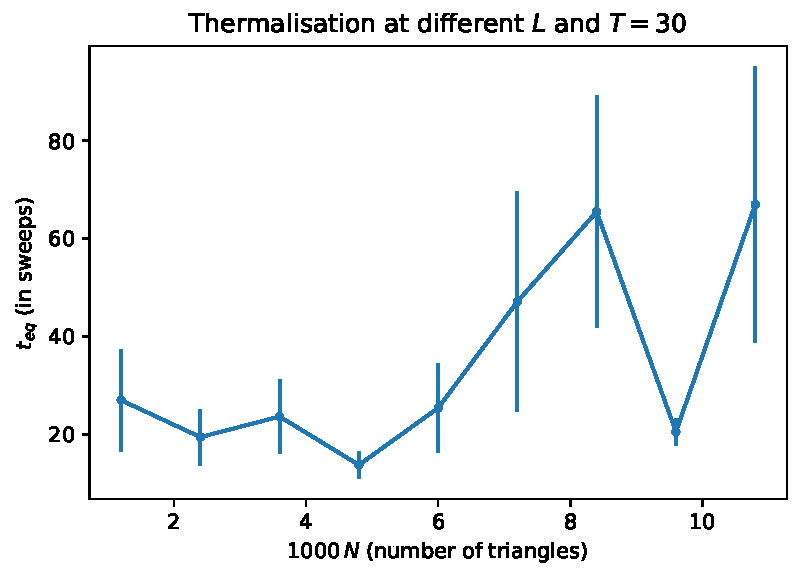
\includegraphics[width=0.95\linewidth]{img/teq-Ldep.pdf}
        \caption{Equilibration time for different sizes of $L$, based on 10 samples for each system size. Determined at move ratio $r=0.4$.}
        \label{fig:teq_Ldep}
    \end{minipage}
\end{figure}

So using this method we can estimate the equilibration time given a trace of $\sigma_\ell$.
Then instead of determining the equilibration time for every system we wish to measure, we attempted to determine the dependence of the equilibration time on different system sizes.
To do this we measured $t_\text{eq}$ for different values of $L$, and to obtain more accurate results and rough estimation of the error the measurements are repeated 10 times for each $L$.
This yields the results presented in Fig. \ref{fig:teq_Ldep} (note that $N = 2 L T$).

The found results show no clear dependence of $t_\text{eq}$ on the system size, and since we only wish to obtain an order estimate of it seems reasonable to assume that \emph{in terms of sweeps} the equilibration time is independent of the system size.
We then take the equilibration time to be $t_\text{eq} = 200 \, \text{sweeps}$ for all simulations to be safe.
This is a very cruse approximation of the equilibration time, but since $200 \,\text{sweeps}$ is not very much it seems unnecessary to put more work in a better estimate of the equilibration time.
%TODO%
% Maybe include the discussion of missing dependence on T for equilibration time?

\paragraph{Autocorrelation}
Once the system has thermalised, we can start to take measurements of the observables of interest.
However, after a single simulation timestep the newly obtained system is still very similar to the previous system, thus observables measured on these systems are by no means independent; they are in fact highly correlated.
Having many correlated measurements is not useful as they do not make the final estimate better, and take up a lot of unnecessary space and computation time.
Moreover, to be able to make and estimate of the error in the final results, it is crucial to know the correlation between measurements.

To estimate the correlation time we will again use the standard deviation as a value is much easier to work with than a function.
The correlation time is then estimated the usual way by determining the autocorrelation of the standard deviation observable over for time:
\begin{equation*}
    \rho(t) = \frac{1}{Z} \, \sum_{i = 1}^{M - t} \qty(\sigma_{\ell, i} - \bar{\sigma}_\ell) \qty(\sigma_{\ell, i + t} - \bar{\sigma}_\ell),
\end{equation*}
where $\sigma_{\ell, i}$ is the $i$th measurement in a set of $M$ measurements of the standard deviation of the length profile, $\bar \sigma_\ell$ is the average standard deviation, and $Z$ is a normalisation factor such that $\rho(0) = 1$.

Now for long enough measurements we expect that the autocorrelation follows exponential decay with which we can define the correlation time $t_\text{cor}$ such that $\rho(t) \approx \exp(- t / t_\text{cor})$.
So to estimate $t_\text{cor}$ we simulate a long trace of $\sigma_\ell$ and fit an exponential decay to the autocorrelation of that trace.
To estimate the error on the estimate of the correlation time we can repeat the measurements several times; or to save on equilibration time we can simulate a very long trace and divide the trace up in batches which we treat as separate measurements.

We would like the autocorrelation to be as small as possible.
So now we have a method of determining the autocorrelation, we can use it to tune the move-ratio $r$ such that the autocorrelation is minimized.
To do this we estimate the autocorrelation for different move ratio's, the results of which are displayed in Fig. \ref{fig:tcor_rdep}.
\begin{figure}[h]
    \centering
    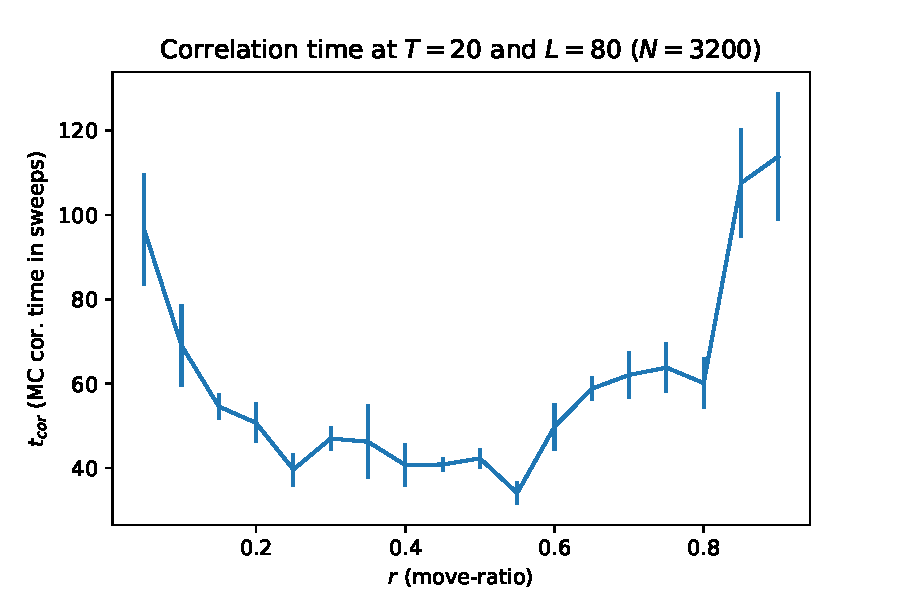
\includegraphics[width=0.7\linewidth]{img/tcor_r_t20_l80.pdf}
    \caption{Correlation time as function of the move-ratio.}
    \label{fig:tcor_rdep}
\end{figure}
From this figure one can clearly see that move ratio's close to $0$ or $1$ have a very long correlation time, which makes sense as both moves are necessary to make the system ergodic such that when only one of the two moves is readily available it takes the system a long time to get to a different state.
From the plot it also seems that the correlation time is not very sensitive to the move ratio, as the correlation time estimate remains roughly constant for ratio's between $0.3$ and $0.5$.
So it seems save to simply pick $r = 0.4$ as there is no need to tune the ratio to a very specific value.

Then finally we wish to estimate the dependence of the correlation time on the system size, such that we can save on storage and computation time.
To do this we estimate the correlation time for multiple system sizes like 


\subsection{Standard deviation}
% Presentation of the results of the standard deviation of the length profile

\subsection{Length correlation}
% Presentation of the results of the analysis of the length correlation of the length profile
\paragraph{Timothy's formula's}
Uit hoofdstuk 4.1 van arXiv:1203.3591 kun je afleiden dat in de continue
limiet met een tijdsinterval T en kosmologische constante $\Lambda$ de
covariantie van de ruimtelijke lengtes $L(t)$ in de limiet $T$ naar oneindig gegeven wordt door
\begin{equation}
    \text{Cov}\big(\ell(0), \ell(t)\big) = \Exp{\ell(0) - L} \Exp{\ell(t) - L}
    = \frac{1}{2\Lambda} e^{- 2\abs{t}\sqrt{\Lambda}}
\end{equation}
terwijl de verwachtingswaarde gelijk is aan
\begin{equation}
    \Exp{\ell(t)} = \frac{1}{\sqrt{\Lambda}} = L
\end{equation}
In deze limiet van grote $T$ is het de verwachting dat het niet veel
uitmaakt of het totale volume vastgezet wordt of dat er een
kosmologische constante genomen wordt (wat is de juiste relatie tussen
volume en $\Lambda$ in dit geval?).

Kun je deze covariantie zien in de data (tenminste voor $\abs{t} \ll T$)? En is
de constante in de e-macht daar ook gerelateerd aan $\Exp{L(t)}$?



\subsection{Discussion}
% Discussion of the interpretation and validity of the results
% Explaination of the difficulties in determining useful results
% Suggestions on improving these measurements